\documentclass[]{book}
\usepackage{lmodern}
\usepackage{amssymb,amsmath}
\usepackage{ifxetex,ifluatex}
\usepackage{fixltx2e} % provides \textsubscript
\ifnum 0\ifxetex 1\fi\ifluatex 1\fi=0 % if pdftex
  \usepackage[T1]{fontenc}
  \usepackage[utf8]{inputenc}
\else % if luatex or xelatex
  \ifxetex
    \usepackage{mathspec}
  \else
    \usepackage{fontspec}
  \fi
  \defaultfontfeatures{Ligatures=TeX,Scale=MatchLowercase}
\fi
% use upquote if available, for straight quotes in verbatim environments
\IfFileExists{upquote.sty}{\usepackage{upquote}}{}
% use microtype if available
\IfFileExists{microtype.sty}{%
\usepackage{microtype}
\UseMicrotypeSet[protrusion]{basicmath} % disable protrusion for tt fonts
}{}
\usepackage{hyperref}
\hypersetup{unicode=true,
            pdftitle={Hurricane Analysis and Visulization Using R},
            pdfauthor={Romane Goldmuntz, Vy Tran, and Jianqiong Zhan},
            pdfborder={0 0 0},
            breaklinks=true}
\urlstyle{same}  % don't use monospace font for urls
\usepackage{natbib}
\bibliographystyle{apalike}
\usepackage{color}
\usepackage{fancyvrb}
\newcommand{\VerbBar}{|}
\newcommand{\VERB}{\Verb[commandchars=\\\{\}]}
\DefineVerbatimEnvironment{Highlighting}{Verbatim}{commandchars=\\\{\}}
% Add ',fontsize=\small' for more characters per line
\usepackage{framed}
\definecolor{shadecolor}{RGB}{248,248,248}
\newenvironment{Shaded}{\begin{snugshade}}{\end{snugshade}}
\newcommand{\AlertTok}[1]{\textcolor[rgb]{0.94,0.16,0.16}{#1}}
\newcommand{\AnnotationTok}[1]{\textcolor[rgb]{0.56,0.35,0.01}{\textbf{\textit{#1}}}}
\newcommand{\AttributeTok}[1]{\textcolor[rgb]{0.77,0.63,0.00}{#1}}
\newcommand{\BaseNTok}[1]{\textcolor[rgb]{0.00,0.00,0.81}{#1}}
\newcommand{\BuiltInTok}[1]{#1}
\newcommand{\CharTok}[1]{\textcolor[rgb]{0.31,0.60,0.02}{#1}}
\newcommand{\CommentTok}[1]{\textcolor[rgb]{0.56,0.35,0.01}{\textit{#1}}}
\newcommand{\CommentVarTok}[1]{\textcolor[rgb]{0.56,0.35,0.01}{\textbf{\textit{#1}}}}
\newcommand{\ConstantTok}[1]{\textcolor[rgb]{0.00,0.00,0.00}{#1}}
\newcommand{\ControlFlowTok}[1]{\textcolor[rgb]{0.13,0.29,0.53}{\textbf{#1}}}
\newcommand{\DataTypeTok}[1]{\textcolor[rgb]{0.13,0.29,0.53}{#1}}
\newcommand{\DecValTok}[1]{\textcolor[rgb]{0.00,0.00,0.81}{#1}}
\newcommand{\DocumentationTok}[1]{\textcolor[rgb]{0.56,0.35,0.01}{\textbf{\textit{#1}}}}
\newcommand{\ErrorTok}[1]{\textcolor[rgb]{0.64,0.00,0.00}{\textbf{#1}}}
\newcommand{\ExtensionTok}[1]{#1}
\newcommand{\FloatTok}[1]{\textcolor[rgb]{0.00,0.00,0.81}{#1}}
\newcommand{\FunctionTok}[1]{\textcolor[rgb]{0.00,0.00,0.00}{#1}}
\newcommand{\ImportTok}[1]{#1}
\newcommand{\InformationTok}[1]{\textcolor[rgb]{0.56,0.35,0.01}{\textbf{\textit{#1}}}}
\newcommand{\KeywordTok}[1]{\textcolor[rgb]{0.13,0.29,0.53}{\textbf{#1}}}
\newcommand{\NormalTok}[1]{#1}
\newcommand{\OperatorTok}[1]{\textcolor[rgb]{0.81,0.36,0.00}{\textbf{#1}}}
\newcommand{\OtherTok}[1]{\textcolor[rgb]{0.56,0.35,0.01}{#1}}
\newcommand{\PreprocessorTok}[1]{\textcolor[rgb]{0.56,0.35,0.01}{\textit{#1}}}
\newcommand{\RegionMarkerTok}[1]{#1}
\newcommand{\SpecialCharTok}[1]{\textcolor[rgb]{0.00,0.00,0.00}{#1}}
\newcommand{\SpecialStringTok}[1]{\textcolor[rgb]{0.31,0.60,0.02}{#1}}
\newcommand{\StringTok}[1]{\textcolor[rgb]{0.31,0.60,0.02}{#1}}
\newcommand{\VariableTok}[1]{\textcolor[rgb]{0.00,0.00,0.00}{#1}}
\newcommand{\VerbatimStringTok}[1]{\textcolor[rgb]{0.31,0.60,0.02}{#1}}
\newcommand{\WarningTok}[1]{\textcolor[rgb]{0.56,0.35,0.01}{\textbf{\textit{#1}}}}
\usepackage{longtable,booktabs}
\usepackage{graphicx,grffile}
\makeatletter
\def\maxwidth{\ifdim\Gin@nat@width>\linewidth\linewidth\else\Gin@nat@width\fi}
\def\maxheight{\ifdim\Gin@nat@height>\textheight\textheight\else\Gin@nat@height\fi}
\makeatother
% Scale images if necessary, so that they will not overflow the page
% margins by default, and it is still possible to overwrite the defaults
% using explicit options in \includegraphics[width, height, ...]{}
\setkeys{Gin}{width=\maxwidth,height=\maxheight,keepaspectratio}
\IfFileExists{parskip.sty}{%
\usepackage{parskip}
}{% else
\setlength{\parindent}{0pt}
\setlength{\parskip}{6pt plus 2pt minus 1pt}
}
\setlength{\emergencystretch}{3em}  % prevent overfull lines
\providecommand{\tightlist}{%
  \setlength{\itemsep}{0pt}\setlength{\parskip}{0pt}}
\setcounter{secnumdepth}{5}
% Redefines (sub)paragraphs to behave more like sections
\ifx\paragraph\undefined\else
\let\oldparagraph\paragraph
\renewcommand{\paragraph}[1]{\oldparagraph{#1}\mbox{}}
\fi
\ifx\subparagraph\undefined\else
\let\oldsubparagraph\subparagraph
\renewcommand{\subparagraph}[1]{\oldsubparagraph{#1}\mbox{}}
\fi

%%% Use protect on footnotes to avoid problems with footnotes in titles
\let\rmarkdownfootnote\footnote%
\def\footnote{\protect\rmarkdownfootnote}

%%% Change title format to be more compact
\usepackage{titling}

% Create subtitle command for use in maketitle
\providecommand{\subtitle}[1]{
  \posttitle{
    \begin{center}\large#1\end{center}
    }
}

\setlength{\droptitle}{-2em}

  \title{Hurricane Analysis and Visulization Using R}
    \pretitle{\vspace{\droptitle}\centering\huge}
  \posttitle{\par}
    \author{Romane Goldmuntz, Vy Tran, and Jianqiong Zhan}
    \preauthor{\centering\large\emph}
  \postauthor{\par}
      \predate{\centering\large\emph}
  \postdate{\par}
    \date{2019-11-07}

\usepackage{booktabs}
\usepackage{amsthm}
\makeatletter
\def\thm@space@setup{%
  \thm@preskip=8pt plus 2pt minus 4pt
  \thm@postskip=\thm@preskip
}
\makeatother

\begin{document}
\maketitle

{
\setcounter{tocdepth}{1}
\tableofcontents
}
\hypertarget{preface}{%
\chapter{Preface}\label{preface}}

This is a class project written in \textbf{Markdown}. We are still working on it.

We are using the \textbf{bookdown} package \citep{R-bookdown} in this project, which was built on top of R Markdown and \textbf{knitr} \citep{xie2015}.

\hypertarget{intro}{%
\chapter{Introduction}\label{intro}}

As coastal shoreline counties create about 40\% of the United States's jobs and account for 46\% of its GDP, hurricanes have a trumendous impact on the country's economy.

They are considered as one of the costliest natural disasters in the world : they currently cost the government over \$28 billion each year, and that amount is expected to increase to over \$39 billion a year due to the increased development of the U.S. coastlines and the global warming. The latter will indeed increase the proportion of cyclones of category 4 and 5, which lead to the most damages and therefore higher costs \citep{Amadeo2019}.

Besides the government, several industries are heavily impacted by hurricanes, including the insurance industry. For example, according to Bloomberg, hurricane Dorian caused the insurance industry losses of up \$25 billion, making it the most expensive natural disaster for the industry since 2017's Hurricane Maria \citep{DSouza2019}.

\begin{Shaded}
\begin{Highlighting}[]
\KeywordTok{library}\NormalTok{(rvest)}
\KeywordTok{library}\NormalTok{(dplyr)}
\KeywordTok{library}\NormalTok{(robotstxt)}
\KeywordTok{library}\NormalTok{(ggplot2)}
\NormalTok{url <-}\StringTok{ "https://en.wikipedia.org/wiki/List_of_costliest_Atlantic_hurricanes"}
\CommentTok{#paths_allowed(url)}

\NormalTok{df<-}\KeywordTok{as.data.frame}\NormalTok{(}\KeywordTok{read_html}\NormalTok{(url) }\OperatorTok\StringTok{ }\KeywordTok{html_table}\NormalTok{(}\DataTypeTok{fill =} \OtherTok{TRUE}\NormalTok{))}

\NormalTok{df_clean <-}\StringTok{ }\NormalTok{df }\OperatorTok\StringTok{ }\KeywordTok{mutate}\NormalTok{(}\DataTypeTok{Nominal_Damage =} \KeywordTok{as.factor}\NormalTok{(}\KeywordTok{gsub}\NormalTok{(}\StringTok{"[$><]"}\NormalTok{, }\StringTok{""}\NormalTok{,Nominal.damage.Billions.USD.)))}\OperatorTok
\StringTok{  }\KeywordTok{select}\NormalTok{(Name, Season, Storm.classificationat.peak.intensity,Nominal_Damage) }\OperatorTok\StringTok{ }\KeywordTok{rename}\NormalTok{(}\DataTypeTok{Classification =}\NormalTok{ Storm.classificationat.peak.intensity)}
\NormalTok{df_clean}\OperatorTok{$}\NormalTok{Season<-}\KeywordTok{as.factor}\NormalTok{(df_clean}\OperatorTok{$}\NormalTok{Season)}
\NormalTok{as.numeric.factor <-}\StringTok{ }\ControlFlowTok{function}\NormalTok{(x) \{}\KeywordTok{as.numeric}\NormalTok{(}\KeywordTok{levels}\NormalTok{(x))[x]\}}
\NormalTok{df_clean[}\DecValTok{4}\NormalTok{]<-}\KeywordTok{lapply}\NormalTok{(df_clean[}\DecValTok{4}\NormalTok{],as.numeric.factor)}
\NormalTok{df_clean[}\DecValTok{2}\NormalTok{]<-}\KeywordTok{lapply}\NormalTok{(df_clean[}\DecValTok{2}\NormalTok{],as.numeric.factor)}
\NormalTok{df_clean <-}\StringTok{ }\NormalTok{df_clean }\OperatorTok\StringTok{ }\KeywordTok{arrange}\NormalTok{(}\KeywordTok{desc}\NormalTok{(Season)) }\OperatorTok\StringTok{ }\KeywordTok{top_n}\NormalTok{(}\DecValTok{6}\NormalTok{)}
\KeywordTok{ggplot}\NormalTok{(df_clean,}\KeywordTok{aes}\NormalTok{(}\DataTypeTok{x=}\NormalTok{Name, }\DataTypeTok{y=}\NormalTok{ Nominal_Damage)) }\OperatorTok{+}\StringTok{ }\KeywordTok{geom_bar}\NormalTok{(}\DataTypeTok{position =} \StringTok{"dodge"}\NormalTok{, }\DataTypeTok{stat =} \StringTok{"identity"}\NormalTok{) }\OperatorTok{+}\StringTok{ }\KeywordTok{coord_flip}\NormalTok{() }\OperatorTok{+}\StringTok{ }\KeywordTok{xlab}\NormalTok{(}\StringTok{"Hurricane"}\NormalTok{) }\OperatorTok{+}\StringTok{ }\KeywordTok{ylab}\NormalTok{(}\StringTok{"Damage (in Billion Dollars)"}\NormalTok{) }\OperatorTok{+}\StringTok{ }\KeywordTok{ggtitle}\NormalTok{(}\StringTok{"Cost of Damage by Six Most Recent Hurricanes"}\NormalTok{) }\OperatorTok{+}\StringTok{ }\KeywordTok{theme_classic}\NormalTok{()}
\end{Highlighting}
\end{Shaded}

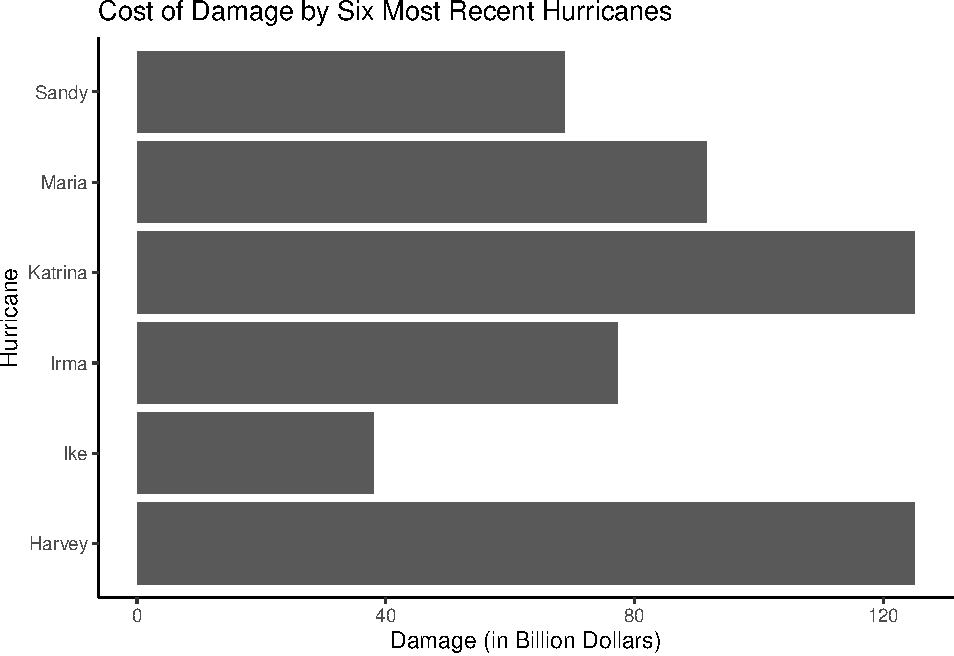
\includegraphics{edav-final-project_files/figure-latex/unnamed-chunk-2-1.pdf}

In addition, hurricane tracking data can provide Federal Emergency Management Agency (FEMA), local emergency managers, and first responders the information they need to be able to send out appropriate responses and help to the citizens at the affected areas \citep{Newtools4H2019}.

For those reasons, hurricanes data is very interesting to analyze and will constitute the topic of this Exploratory Data Analysis and Vizualisation final project.

\hypertarget{methods}{%
\chapter{Methods}\label{methods}}

\hypertarget{data-sources}{%
\section{Data sources}\label{data-sources}}

(We describe our data sources, our methods in this chapter)

Storm tracks data can be downloaded from \href{https://www.nhc.noaa.gov/data/\#hurdat}{National Hurricane Center and Central Pacific Hurricane Center}. The data using in the project is known as Atlantic hurricane database (\href{https://www.nhc.noaa.gov/data/hurdat/hurdat2-format-atlantic.pdf}{HURDAT2}) 1851-2018 (\href{https://www.nhc.noaa.gov/data/hurdat/hurdat2-1851-2018-051019.txt}{5.9MB download}). The data has a comma-delimited, text format with six-hourly information on the location, maximum winds, central pressure, and (beginning in 2004) size of all known tropical cyclones and subtropical cyclones.

\hypertarget{data-transformat}{%
\section{Data transformat}\label{data-transformat}}

Describe the process of getting the data into a form in which you could work with it in R.

\begin{Shaded}
\begin{Highlighting}[]
\KeywordTok{library}\NormalTok{(tidyverse)}
\KeywordTok{library}\NormalTok{(stringr)}
\CommentTok{# Read in data set}
\CommentTok{#dfile <- read_lines("https://www.nhc.noaa.gov/data/hurdat/hurdat2-1851-2018-051019.txt")}
\NormalTok{dfile<-}\StringTok{ "data/hurdat2-1851-2018-051019.txt"}
\NormalTok{storm_strings <-}\StringTok{ }\KeywordTok{read_lines}\NormalTok{(dfile)}
\end{Highlighting}
\end{Shaded}

\begin{Shaded}
\begin{Highlighting}[]
\CommentTok{# Identify the header lines that have three commas}
\KeywordTok{library}\NormalTok{(stringr)}
\NormalTok{header_locations <-}\StringTok{ }\NormalTok{(}\DecValTok{1}\OperatorTok{:}\KeywordTok{length}\NormalTok{(storm_strings))[}\KeywordTok{str_count}\NormalTok{(storm_strings, }\StringTok{"}\CharTok{\textbackslash{}\textbackslash{}}\StringTok{,"}\NormalTok{) }\OperatorTok{==}\StringTok{ }\DecValTok{3}\NormalTok{] }\CommentTok{# count # of strings for each line, the header line has only 3 strings.}

\NormalTok{headers <-}\StringTok{ }\KeywordTok{as.list}\NormalTok{(storm_strings[header_locations])}
\NormalTok{headers_df <-}\StringTok{ }
\StringTok{  }\NormalTok{headers }\OperatorTok
\StringTok{  }\NormalTok{purrr}\OperatorTok{::}\KeywordTok{map}\NormalTok{(stringr}\OperatorTok{::}\NormalTok{str_sub, }\DataTypeTok{start =}\NormalTok{ 1L, }\DataTypeTok{end =} \OperatorTok{-}\NormalTok{2L) }\OperatorTok\StringTok{ }\CommentTok{# to remove trailing comma}
\StringTok{  }\NormalTok{purrr}\OperatorTok{::}\KeywordTok{map}\NormalTok{(paste0, }\StringTok{"}\CharTok{\textbackslash{}n}\StringTok{"}\NormalTok{) }\OperatorTok\StringTok{                 }\CommentTok{# and replace final comma with \textbackslash{}n}
\StringTok{  }\NormalTok{purrr}\OperatorTok{::}\KeywordTok{map_dfr}\NormalTok{(read_csv, }\DataTypeTok{col_names =} \KeywordTok{c}\NormalTok{(}\StringTok{"id"}\NormalTok{, }\StringTok{"name"}\NormalTok{, }\StringTok{"n_obs"}\NormalTok{)) }\OperatorTok
\StringTok{  }\NormalTok{dplyr}\OperatorTok{::}\KeywordTok{mutate}\NormalTok{(}\CommentTok{#name = dplyr::recode(name, "UNNAMED" = id), }
                \DataTypeTok{skip =}\NormalTok{ header_locations) }\OperatorTok
\StringTok{  }\NormalTok{dplyr}\OperatorTok{::}\KeywordTok{select}\NormalTok{(id, name, skip, n_obs)}
\end{Highlighting}
\end{Shaded}

\begin{Shaded}
\begin{Highlighting}[]
\CommentTok{# Set data frames names}
\NormalTok{df_names <-}\StringTok{ }\KeywordTok{c}\NormalTok{(}
  \StringTok{"date"}\NormalTok{, }\StringTok{"time"}\NormalTok{, }\StringTok{"record_type"}\NormalTok{, }\StringTok{"status"}\NormalTok{, }\StringTok{"lat"}\NormalTok{, }\StringTok{"long"}\NormalTok{, }\StringTok{"wind"}\NormalTok{, }\StringTok{"pressure"}\NormalTok{,}
  \StringTok{"extent_34_NE"}\NormalTok{, }\StringTok{"extent_34_SE"}\NormalTok{, }\StringTok{"extent_34_SW"}\NormalTok{, }\StringTok{"extent_34_NW"}\NormalTok{,}
  \StringTok{"extent_50_NE"}\NormalTok{, }\StringTok{"extent_50_SE"}\NormalTok{, }\StringTok{"extent_50_SW"}\NormalTok{, }\StringTok{"extent_50_NW"}\NormalTok{,}
  \StringTok{"extent_64_NE"}\NormalTok{, }\StringTok{"extent_64_SE"}\NormalTok{, }\StringTok{"extent_64_SW"}\NormalTok{, }\StringTok{"extent_64_NW"}\NormalTok{, }\StringTok{"nas"}
\NormalTok{)}

\NormalTok{storm_dfs <-}\StringTok{ }\KeywordTok{vector}\NormalTok{(}\StringTok{"list"}\NormalTok{, }\KeywordTok{nrow}\NormalTok{(headers_df))}
\KeywordTok{names}\NormalTok{(storm_dfs) <-}\StringTok{ }\NormalTok{headers_df}\OperatorTok{$}\NormalTok{id}
\end{Highlighting}
\end{Shaded}

\begin{Shaded}
\begin{Highlighting}[]
\CommentTok{# Read in the sub-datasets as data frames}
\ControlFlowTok{for}\NormalTok{ (i }\ControlFlowTok{in} \KeywordTok{seq_along}\NormalTok{(headers_df}\OperatorTok{$}\NormalTok{name)) \{}
\NormalTok{  storm_dfs[[i]] <-}\StringTok{ }\KeywordTok{read_csv}\NormalTok{(dfile,}
    \DataTypeTok{skip =}\NormalTok{ headers_df}\OperatorTok{$}\NormalTok{skip[i],}
    \DataTypeTok{n_max =}\NormalTok{ headers_df}\OperatorTok{$}\NormalTok{n_obs[i],}
    \DataTypeTok{col_names =}\NormalTok{ df_names,}
    \DataTypeTok{na =} \KeywordTok{c}\NormalTok{(}\StringTok{""}\NormalTok{, }\StringTok{"-99"}\NormalTok{, }\StringTok{"-999"}\NormalTok{),}
    \DataTypeTok{col_types =} \KeywordTok{list}\NormalTok{(}
      \DataTypeTok{time =} \KeywordTok{col_character}\NormalTok{(),}
      \DataTypeTok{pressure =} \KeywordTok{col_integer}\NormalTok{(),}
      \DataTypeTok{extent_34_NE =} \KeywordTok{col_integer}\NormalTok{(),}
      \DataTypeTok{extent_34_SE =} \KeywordTok{col_integer}\NormalTok{(),}
      \DataTypeTok{extent_34_SW =} \KeywordTok{col_integer}\NormalTok{(),}
      \DataTypeTok{extent_34_NW =} \KeywordTok{col_integer}\NormalTok{(),}
      \DataTypeTok{extent_50_NE =} \KeywordTok{col_integer}\NormalTok{(),}
      \DataTypeTok{extent_50_SE =} \KeywordTok{col_integer}\NormalTok{(),}
      \DataTypeTok{extent_50_SW =} \KeywordTok{col_integer}\NormalTok{(),}
      \DataTypeTok{extent_50_NW =} \KeywordTok{col_integer}\NormalTok{(),}
      \DataTypeTok{extent_64_NE =} \KeywordTok{col_integer}\NormalTok{(),}
      \DataTypeTok{extent_64_SE =} \KeywordTok{col_integer}\NormalTok{(),}
      \DataTypeTok{extent_64_SW =} \KeywordTok{col_integer}\NormalTok{(),}
      \DataTypeTok{extent_64_NW =} \KeywordTok{col_integer}\NormalTok{()}
\NormalTok{    )}
\NormalTok{  )}
\NormalTok{\}}
\end{Highlighting}
\end{Shaded}

\begin{Shaded}
\begin{Highlighting}[]
\CommentTok{# Combine and clean the data sets}
\KeywordTok{library}\NormalTok{(lubridate)}
\NormalTok{storms <-}\StringTok{ }
\StringTok{  }\NormalTok{storm_dfs }\OperatorTok
\StringTok{  }\NormalTok{dplyr}\OperatorTok{::}\KeywordTok{bind_rows}\NormalTok{(}\DataTypeTok{.id =} \StringTok{"id"}\NormalTok{) }\OperatorTok
\StringTok{  }\NormalTok{dplyr}\OperatorTok{::}\KeywordTok{mutate}\NormalTok{(}
    \DataTypeTok{date =}\NormalTok{ lubridate}\OperatorTok{::}\KeywordTok{ymd}\NormalTok{(date),}
    \DataTypeTok{year =}\NormalTok{ lubridate}\OperatorTok{::}\KeywordTok{year}\NormalTok{(date),}
    \DataTypeTok{month =}\NormalTok{ lubridate}\OperatorTok{::}\KeywordTok{month}\NormalTok{(date),}
    \DataTypeTok{day =}\NormalTok{ lubridate}\OperatorTok{::}\KeywordTok{day}\NormalTok{(date),}
    \DataTypeTok{hour =} \KeywordTok{as.numeric}\NormalTok{(stringr}\OperatorTok{::}\KeywordTok{str_sub}\NormalTok{(time, }\DecValTok{1}\NormalTok{, }\DecValTok{2}\NormalTok{)),}
    \DataTypeTok{datetime =} \KeywordTok{ISOdate}\NormalTok{(year, month, day, hour, }\DataTypeTok{min =} \DecValTok{0}\NormalTok{, }\DataTypeTok{sec =} \DecValTok{0}\NormalTok{, }\DataTypeTok{tz =} \StringTok{"GMT"}\NormalTok{),}
    \DataTypeTok{lat_hemisphere =}\NormalTok{ stringr}\OperatorTok{::}\KeywordTok{str_sub}\NormalTok{(lat, }\DecValTok{-1}\NormalTok{),}
    \DataTypeTok{lat_sign =}\NormalTok{ dplyr}\OperatorTok{::}\KeywordTok{if_else}\NormalTok{(lat_hemisphere }\OperatorTok{==}\StringTok{ "N"}\NormalTok{, }\DecValTok{1}\NormalTok{, }\DecValTok{-1}\NormalTok{),}
    \DataTypeTok{lat =} \KeywordTok{as.numeric}\NormalTok{(stringr}\OperatorTok{::}\KeywordTok{str_sub}\NormalTok{(lat, }\DecValTok{1}\NormalTok{, }\DecValTok{-2}\NormalTok{)) }\OperatorTok{*}\StringTok{ }\NormalTok{lat_sign,}
    \DataTypeTok{long_hemisphere =}\NormalTok{ stringr}\OperatorTok{::}\KeywordTok{str_sub}\NormalTok{(long, }\DecValTok{-1}\NormalTok{),}
    \DataTypeTok{long_sign =}\NormalTok{ dplyr}\OperatorTok{::}\KeywordTok{if_else}\NormalTok{(long_hemisphere }\OperatorTok{==}\StringTok{ "E"}\NormalTok{, }\DecValTok{1}\NormalTok{, }\DecValTok{-1}\NormalTok{),}
    \DataTypeTok{long =} \KeywordTok{as.numeric}\NormalTok{(stringr}\OperatorTok{::}\KeywordTok{str_sub}\NormalTok{(long, }\DecValTok{1}\NormalTok{, }\DecValTok{-2}\NormalTok{)) }\OperatorTok{*}\StringTok{ }\NormalTok{long_sign,}
    \DataTypeTok{category =} \KeywordTok{cut}\NormalTok{(wind, }\CommentTok{#cut divides the range of x into intervals}
      \DataTypeTok{breaks =} \KeywordTok{c}\NormalTok{(}\DecValTok{0}\NormalTok{, }\DecValTok{34}\NormalTok{, }\DecValTok{64}\NormalTok{, }\DecValTok{83}\NormalTok{, }\DecValTok{96}\NormalTok{, }\DecValTok{113}\NormalTok{, }\DecValTok{137}\NormalTok{, }\DecValTok{500}\NormalTok{),}
      \DataTypeTok{labels =} \KeywordTok{c}\NormalTok{(}\OperatorTok{-}\DecValTok{1}\NormalTok{, }\DecValTok{0}\NormalTok{, }\DecValTok{1}\NormalTok{, }\DecValTok{2}\NormalTok{, }\DecValTok{3}\NormalTok{, }\DecValTok{4}\NormalTok{, }\DecValTok{5}\NormalTok{),}
      \DataTypeTok{include.lowest =} \OtherTok{TRUE}\NormalTok{, }\DataTypeTok{ordered =} \OtherTok{TRUE}
\NormalTok{    ),}
    \CommentTok{# wind = wind * 1.15078, # transforms knots to mph,}
    \DataTypeTok{TSradius1 =}\NormalTok{ extent_}\DecValTok{34}\NormalTok{_NE }\OperatorTok{+}\StringTok{ }\NormalTok{extent_}\DecValTok{34}\NormalTok{_SW,}
    \DataTypeTok{TSradius2 =}\NormalTok{ extent_}\DecValTok{34}\NormalTok{_NW }\OperatorTok{+}\StringTok{ }\NormalTok{extent_}\DecValTok{34}\NormalTok{_SE,}
    \DataTypeTok{ts_diameter =} \KeywordTok{pmax}\NormalTok{(TSradius1, TSradius2) }\OperatorTok{*}\StringTok{ }\FloatTok{1.15078}\NormalTok{, }\CommentTok{# to convert from nautical miles to miles # pmax: returns the parallel maxima and minima of the input values}
    \DataTypeTok{HUradius1 =}\NormalTok{ extent_}\DecValTok{64}\NormalTok{_NE }\OperatorTok{+}\StringTok{ }\NormalTok{extent_}\DecValTok{64}\NormalTok{_SW,}
    \DataTypeTok{HUradius2 =}\NormalTok{ extent_}\DecValTok{64}\NormalTok{_NW }\OperatorTok{+}\StringTok{ }\NormalTok{extent_}\DecValTok{64}\NormalTok{_SE,}
    \DataTypeTok{hu_diameter =} \KeywordTok{pmax}\NormalTok{(HUradius1, HUradius2) }\OperatorTok{*}\StringTok{ }\FloatTok{1.15078}\NormalTok{, }\CommentTok{# to convert from nautical miles to miles}
    \DataTypeTok{status =} \KeywordTok{recode}\NormalTok{(status,}
                    \StringTok{"TD"}\NormalTok{ =}\StringTok{ "tropical depression"}\NormalTok{,}
                    \StringTok{"TS"}\NormalTok{ =}\StringTok{ "tropical storm"}\NormalTok{, }
                    \StringTok{"HU"}\NormalTok{ =}\StringTok{ "tropical hurricane"}\NormalTok{, }
                    \StringTok{"EX"}\NormalTok{ =}\StringTok{ "Extratropical cyclone"}\NormalTok{, }\CommentTok{##}
                    \StringTok{"SD"}\NormalTok{ =}\StringTok{ "subtropical depression"}\NormalTok{,}
                    \StringTok{"SS"}\NormalTok{ =}\StringTok{ "subtropical storm"}\NormalTok{, }
                    \StringTok{"HU"}\NormalTok{ =}\StringTok{ "tropical hurricane"}\NormalTok{, }
                    \StringTok{"LO"}\NormalTok{ =}\StringTok{ "a low"}\NormalTok{,}
                    \StringTok{"WV"}\NormalTok{ =}\StringTok{ "tropical wave"}\NormalTok{,}
                    \StringTok{"DB"}\NormalTok{ =}\StringTok{ "disturbance"}\NormalTok{)}
\NormalTok{  ) }
\end{Highlighting}
\end{Shaded}

\begin{Shaded}
\begin{Highlighting}[]
\CommentTok{# data output}
\NormalTok{headers_df_selected <-}\StringTok{ }\NormalTok{headers_df }\OperatorTok\StringTok{ }\KeywordTok{select}\NormalTok{(}\KeywordTok{c}\NormalTok{(}\StringTok{"id"}\NormalTok{,}\StringTok{"name"}\NormalTok{))}
\CommentTok{# headers_df_selected}
\NormalTok{storms_with_name <-}\StringTok{ }\KeywordTok{left_join}\NormalTok{(headers_df_selected, storms, }\DataTypeTok{by=}\KeywordTok{c}\NormalTok{(}\StringTok{"id"}\NormalTok{)) }\OperatorTok\StringTok{ }
\StringTok{  }\KeywordTok{select}\NormalTok{(id, name, datetime, year, month, day, hour, lat, long, status, category,}
\NormalTok{         wind, pressure, }
\NormalTok{         extent_}\DecValTok{34}\NormalTok{_NE, extent_}\DecValTok{34}\NormalTok{_SW, extent_}\DecValTok{34}\NormalTok{_NW, extent_}\DecValTok{34}\NormalTok{_SE,}
\NormalTok{         extent_}\DecValTok{50}\NormalTok{_NE, extent_}\DecValTok{50}\NormalTok{_SW, extent_}\DecValTok{50}\NormalTok{_NW, extent_}\DecValTok{50}\NormalTok{_SE,}
\NormalTok{         extent_}\DecValTok{64}\NormalTok{_NE, extent_}\DecValTok{64}\NormalTok{_SW, extent_}\DecValTok{64}\NormalTok{_NW, extent_}\DecValTok{64}\NormalTok{_SE,}
\NormalTok{         ts_diameter, hu_diameter)}
\end{Highlighting}
\end{Shaded}

\begin{Shaded}
\begin{Highlighting}[]
\NormalTok{storms_all <-}\StringTok{ }\NormalTok{storms_with_name }\OperatorTok\StringTok{ }
\StringTok{  }\KeywordTok{mutate}\NormalTok{(}\DataTypeTok{name=}\NormalTok{ dplyr}\OperatorTok{::}\KeywordTok{if_else}\NormalTok{(}\KeywordTok{grepl}\NormalTok{(}\StringTok{"UNNAMED"}\NormalTok{, name), name,}
\NormalTok{                              stringr}\OperatorTok{::}\KeywordTok{str_to_title}\NormalTok{(name)))}
\end{Highlighting}
\end{Shaded}

\begin{Shaded}
\begin{Highlighting}[]
\NormalTok{storms_all}\OperatorTok{$}\NormalTok{status <-}\StringTok{ }\KeywordTok{factor}\NormalTok{(storms_all}\OperatorTok{$}\NormalTok{status)}
\NormalTok{storms_all}\OperatorTok{$}\NormalTok{id <-}\StringTok{ }\KeywordTok{factor}\NormalTok{(storms_all}\OperatorTok{$}\NormalTok{id)}
\NormalTok{storms_all}\OperatorTok{$}\NormalTok{name <-}\StringTok{ }\KeywordTok{factor}\NormalTok{(storms_all}\OperatorTok{$}\NormalTok{name)}
\end{Highlighting}
\end{Shaded}

\begin{Shaded}
\begin{Highlighting}[]
\KeywordTok{levels}\NormalTok{(storms_all}\OperatorTok{$}\NormalTok{status)}
\end{Highlighting}
\end{Shaded}

\begin{verbatim}
##  [1] "a low"                  "disturbance"            "ET"                    
##  [4] "Extratropical cyclone"  "subtropical depression" "subtropical storm"     
##  [7] "tropical depression"    "tropical hurricane"     "tropical storm"        
## [10] "tropical wave"
\end{verbatim}

\begin{Shaded}
\begin{Highlighting}[]
\NormalTok{storms_all }\OperatorTok\StringTok{ }\KeywordTok{filter}\NormalTok{(status }\OperatorTok{==}\StringTok{ "ET"}\NormalTok{)}
\end{Highlighting}
\end{Shaded}

\begin{verbatim}
## # A tibble: 1 x 27
##   id    name  datetime             year month   day  hour   lat  long status
##   <fct> <fct> <dttm>              <dbl> <dbl> <int> <dbl> <dbl> <dbl> <fct> 
## 1 AL09~ Harv~ 1993-09-21 18:00:00  1993     9    21    18    46   -42 ET    
## # ... with 17 more variables: category <ord>, wind <dbl>, pressure <int>,
## #   extent_34_NE <int>, extent_34_SW <int>, extent_34_NW <int>,
## #   extent_34_SE <int>, extent_50_NE <int>, extent_50_SW <int>,
## #   extent_50_NW <int>, extent_50_SE <int>, extent_64_NE <int>,
## #   extent_64_SW <int>, extent_64_NW <int>, extent_64_SE <int>,
## #   ts_diameter <dbl>, hu_diameter <dbl>
\end{verbatim}

\emph{Note: there is an ``ET'' in \emph{Status of system}, however, there is no description in \href{https://www.nhc.noaa.gov/data/hurdat/hurdat2-format-atlantic.pdf}{HURDAT2}, which is a typo in the dataset, \texttt{recode} it into 'EX".}

\begin{Shaded}
\begin{Highlighting}[]
\NormalTok{storms_all}\OperatorTok{$}\NormalTok{status <-}\StringTok{ }\NormalTok{dplyr}\OperatorTok{::}\KeywordTok{recode}\NormalTok{(storms_all}\OperatorTok{$}\NormalTok{status, }\DataTypeTok{ET =} \StringTok{"Extratropical cyclone"}\NormalTok{)}
\CommentTok{#levels(factor(storms_all$status))}
\end{Highlighting}
\end{Shaded}

\textbf{Narrow to storms that have complete pressure record}

\begin{Shaded}
\begin{Highlighting}[]
\CommentTok{# Narrow to storms that have complete pressure record}
\NormalTok{completeish <-}\StringTok{ }\NormalTok{storms_all }\OperatorTok
\StringTok{  }\NormalTok{dplyr}\OperatorTok{::}\KeywordTok{group_by}\NormalTok{(id) }\OperatorTok
\StringTok{  }\NormalTok{dplyr}\OperatorTok{::}\KeywordTok{summarise}\NormalTok{(}\DataTypeTok{n_pressure =} \KeywordTok{sum}\NormalTok{(}\OperatorTok{!}\KeywordTok{is.na}\NormalTok{(pressure)), }\DataTypeTok{p_pressure =} \KeywordTok{mean}\NormalTok{(}\OperatorTok{!}\KeywordTok{is.na}\NormalTok{(pressure))) }\OperatorTok
\StringTok{  }\NormalTok{dplyr}\OperatorTok{::}\KeywordTok{filter}\NormalTok{(p_pressure }\OperatorTok{==}\StringTok{ }\DecValTok{1}\NormalTok{) }\OperatorTok
\StringTok{  }\NormalTok{.[[}\StringTok{"id"}\NormalTok{]]}
\CommentTok{#length(completeish)}
\KeywordTok{dim}\NormalTok{(storms_all)[}\DecValTok{1}\NormalTok{]}
\end{Highlighting}
\end{Shaded}

\begin{verbatim}
## [1] 50911
\end{verbatim}

Theare are 562 out of 50911storms that have complete pressure record.

\begin{Shaded}
\begin{Highlighting}[]
\NormalTok{storms_completish_selected <-}\StringTok{ }\NormalTok{storms_all }\OperatorTok
\StringTok{  }\KeywordTok{filter}\NormalTok{(}
\NormalTok{    status }\OperatorTok\StringTok{ }\KeywordTok{c}\NormalTok{(}\StringTok{"hurricane"}\NormalTok{, }\StringTok{"tropical storm"}\NormalTok{, }\StringTok{"tropical depression"}\NormalTok{),}
\NormalTok{    id }\OperatorTok\StringTok{ }\NormalTok{completeish)}
\end{Highlighting}
\end{Shaded}

\begin{Shaded}
\begin{Highlighting}[]
\NormalTok{storms_all_add_com <-}\StringTok{ }\NormalTok{storms_all }\OperatorTok\StringTok{ }\KeywordTok{mutate}\NormalTok{(}\DataTypeTok{completeish =} \KeywordTok{if_else}\NormalTok{(status }\OperatorTok\StringTok{ }\KeywordTok{c}\NormalTok{(}\StringTok{"hurricane"}\NormalTok{, }\StringTok{"tropical storm"}\NormalTok{, }\StringTok{"tropical depression"}\NormalTok{) }\OperatorTok{&}\StringTok{ }\NormalTok{id }\OperatorTok\StringTok{ }\NormalTok{completeish, }\StringTok{"yes"}\NormalTok{,}\StringTok{"no"}\NormalTok{))}
\NormalTok{storms_all_add_com}\OperatorTok{$}\NormalTok{completeish <-}\StringTok{ }\KeywordTok{factor}\NormalTok{(storms_all_add_com}\OperatorTok{$}\NormalTok{completeish)}
\end{Highlighting}
\end{Shaded}

\textbf{Save tranformed data}

\begin{Shaded}
\begin{Highlighting}[]
\NormalTok{dir <-}\StringTok{ 'data/'}
\KeywordTok{write_csv}\NormalTok{(storms_all_add_com, }\KeywordTok{file.path}\NormalTok{(dir, }\StringTok{"storms_all_out.csv"}\NormalTok{))}
\end{Highlighting}
\end{Shaded}

\begin{Shaded}
\begin{Highlighting}[]
\NormalTok{dir <-}\StringTok{ 'data/'}
\KeywordTok{write_csv}\NormalTok{(storms, }\KeywordTok{file.path}\NormalTok{(dir, }\StringTok{"storms_completish_selected.csv"}\NormalTok{))}
\end{Highlighting}
\end{Shaded}

\hypertarget{missing-values}{%
\section{Missing values}\label{missing-values}}

Describe any patterns you discover in missing values.

\hypertarget{results}{%
\chapter{Results}\label{results}}

Provide a short nontechnical but \emph{significant} summary of the most revealing findings of our analysis written for a nontechnical audience. Take extra care to clean up our graphs, ensuring that best practices for presentation are followed, as described in the audience ready style section below.

\hypertarget{interactive-component}{%
\chapter{Interactive Component}\label{interactive-component}}

Select one (or more) of our key findings to present in an interactive format (D3). Be selective in the choices that we present to the user; the idea is that in 5-10 minutes, users should have a good sense of the question(s) that we are interested in and the trends we've identified in the data. In other words, they should understand the value of the analysis, be it business value, scientific value, general knowledge, etc.

\#\texttt{\{r\ out.width=\textquotesingle{}100\%\textquotesingle{},\ echo=FALSE\}\ library(leaflet)\ leaflet()\ \%\textgreater{}\%\ addTiles()\ \%\textgreater{}\%\ \ \ setView(-93.65,\ 42.0285,\ zoom\ =\ 17)\ \%\textgreater{}\%\ \ \ addPopups(\ \ \ \ \ -93.65,\ 42.0285,\ \ \ \ \ \textquotesingle{}Here\ is\ the\ \textless{}b\textgreater{}Department\ of\ Statistics\textless{}/b\textgreater{},\ ISU\textquotesingle{}\ \ \ )\ \#}
\#\texttt{\{r\}\ \#devtools::install\_github("rstudio/r2d3",\ force\ =\ TRUE)}

\#\texttt{\{r\}\ library(r2d3)\ r2d3(data=c(0.3,\ 0.6,\ 0.8,\ 0.95,\ 0.40,\ 0.20),\ script\ =\ "barchart.js")\ \#}

\hypertarget{conclusion}{%
\chapter{Conclusion}\label{conclusion}}

Discuss limitations and future directions, lessons learned.

\bibliography{proj.bib,packages.bib}


\end{document}
